\chapter{Introduction à Factorio}
\section{Pourquoi utiliser Factorio?}
	
\subsection{Qu'est-ce-que Factorio?} 

\paragraph{}

\textbf{Factorio} un jeu de logistique, stratégie, résolution de problèmes et de gestion de ressources fortement inspiré des packs de mods \textbf{Feed The Beast (FTB)} pour le jeu \textbf{Minecraft}, où le joueur doit automatiser la production et la transformation de ressources afin de pouvoir progresser dans le jeu par le biais de tapis roulants, de trains, de logique et de machines.

\begin{figure}[h]
\centering
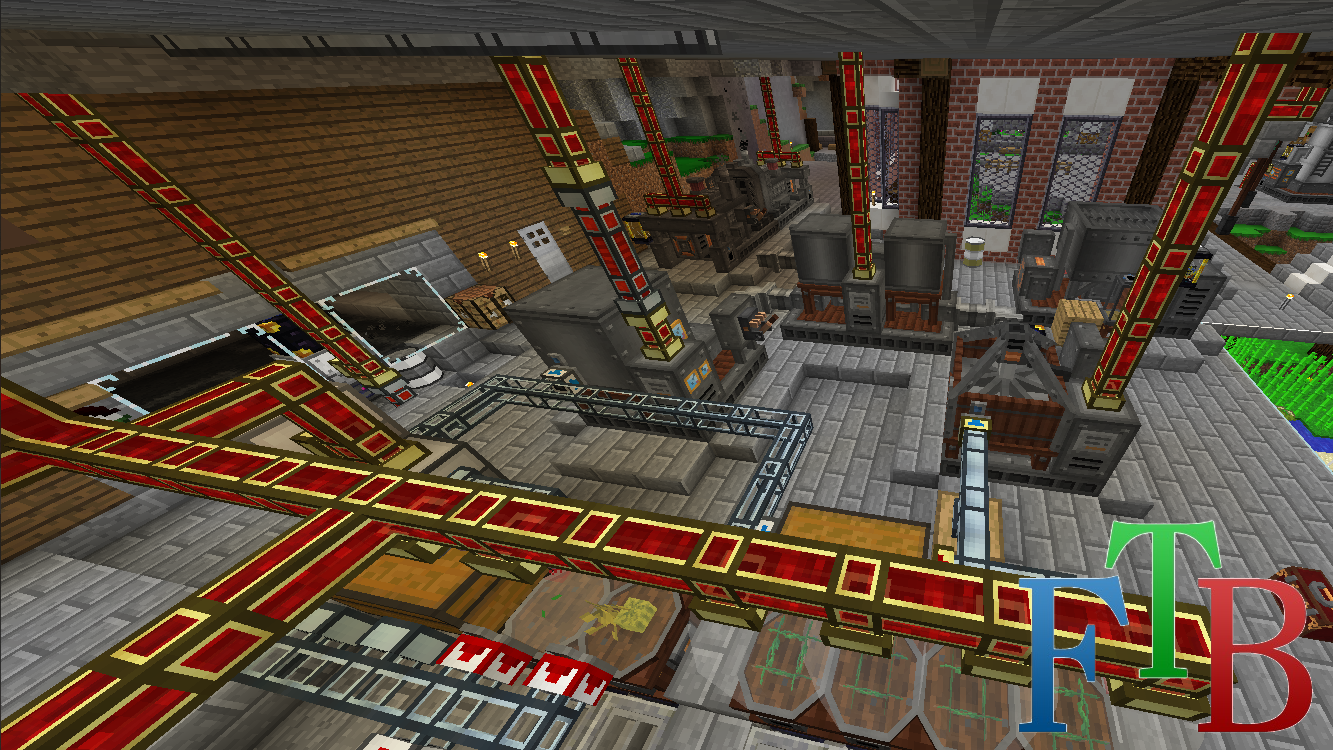
\includegraphics[width=0.8\linewidth]{pics/ftb-presentation.png}

\caption{Exemple d'automatisation Feed The Beast}
\end{figure}

\begin{figure}[h]
\centering
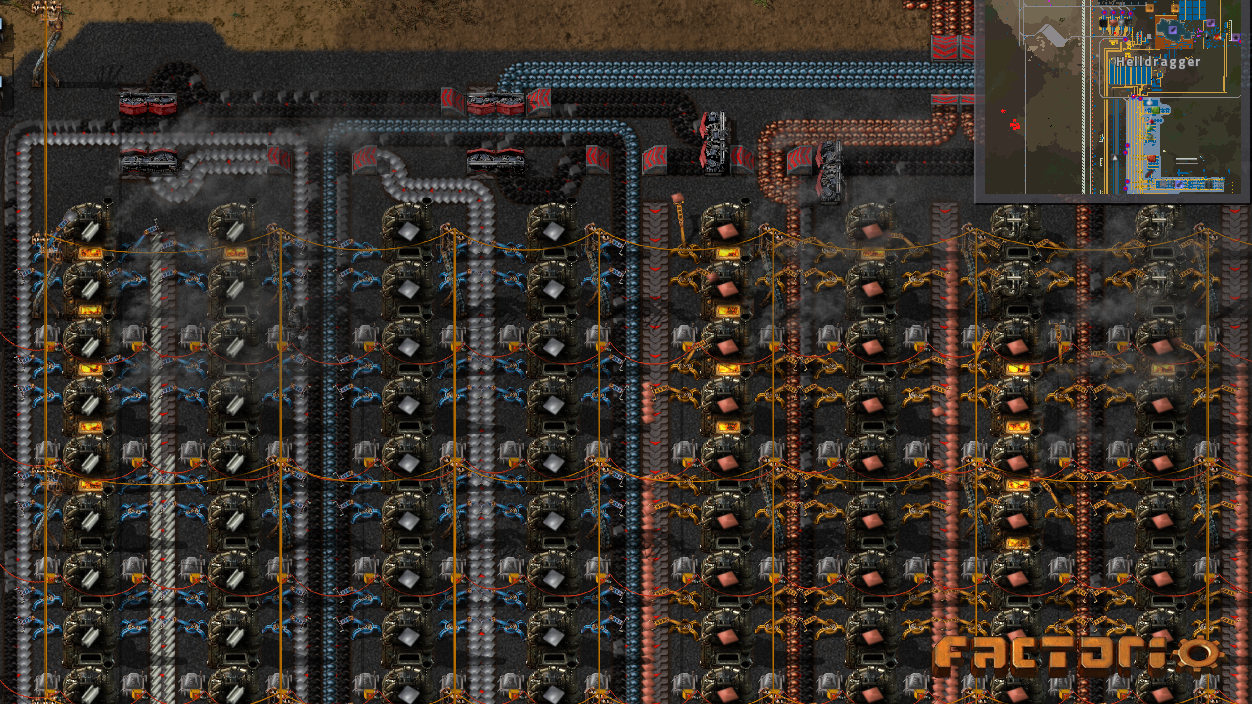
\includegraphics[width=0.8\linewidth]{pics/factorio-presentation.png}

\caption{Exemple d'automatisation Factorio}
\end{figure}


Ce jeu en particulier présente au joueur la mécanique de jeu du réseau logique qui permet à chaque itération du moteur de jeu de transmettre des signaux spécifiques pouvant avoir pour toute valeur entière signée sur 32 bits.
À cela s'ajoute la présence de méthodes d'utilisation et d'évaluations de ces signaux qui permettent de réaliser des systèmes d'automatisation logique et complexes, notamment les combinateurs arithmétiques et combinateurs logiques que nous allons voir plus en détails plus bas.


\begin{figure}[h]
\centering
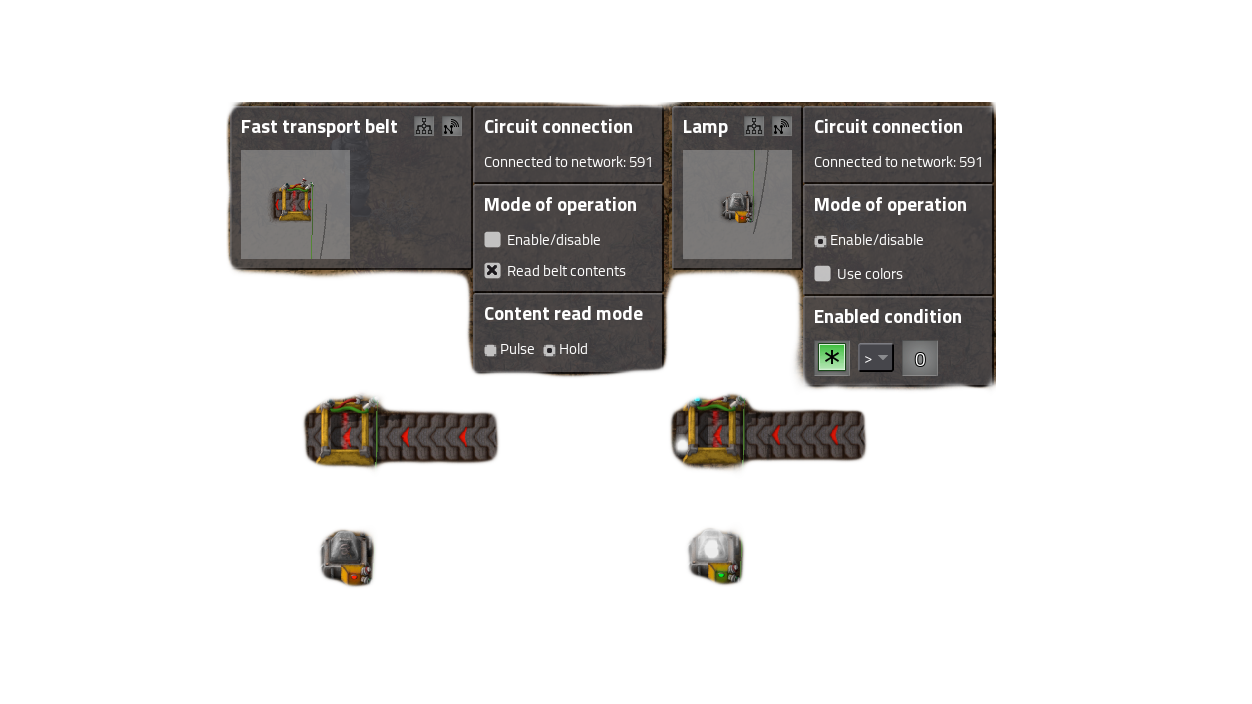
\includegraphics[width=0.8\linewidth]{pics/factorio-logic-basis.png}

\captionof{figure}{Exemple de logique  basique: Détecteur d'objet}
\end{figure}

Le jeu lui même intègre aussi un système de \textbf{blueprint}, des plans de constructions récupérable et partageable hors du jeu permettant de construire divers systèmes complexes entre joueurs.


\subsection{Les circuits logiques}

\paragraph{Les réseaux logiques} 
sont construits en utilisant des câbles rouge ou vert, et permettent le contrôle de récepteurs, basé sur les informations envoyées sur le réseau par les émetteurs connectés. 
La plupart des émetteurs sont des périphériques de stockage, et émettent les informations de leur contenu sur des signaux spécifiques, basés sur le type des objets ou fluides que le périphérique de stockage contient. 

Chaque réseau logique contient un signal pour chaque type d'objet du jeu, ainsi que 45 signaux virtuels supplémentaires qui agissent en tant que signaux définis par le joueur. 
Les signaux spéciaux ['Tout'], ['N'importe quoi'] et ['Chacun'] sont aussi disponibles.

\subsection{Les signaux virtuels logiques}

\begin{minipage}[t]{\textwidth}

{
\centering
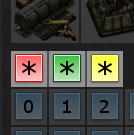
\includegraphics{pics/factorio-logic-signals.png}
\captionof{figure}{Les signaux [Tout], [N'importe quoi] et [Chacun] respectivement}
}


\end{minipage} 

\paragraph{[Tout]}
peut être utilisé sur la partie gauche des conditionnels. 
Cette condition sera vraie si la condition est vraie pour tous les signaux en entrée. 
La condition est aussi vraie en l'absence de tout signal. 
Cela signifie que le signal [Tout] se comporte comme une \textbf{quantification universelle}.

La sortie d'un comparateur peut aussi utiliser [Tout]. 
Quand ce signal est utilisé en sortie, cela signifie que le comparateur va faire passer tous les signaux qui remplissent la condition déterminée.  

\paragraph{[N'importe quoi]} 
peut être utilisé sur la partie gauche des conditionnels. 
La condition est vraie quand elle est vérifiée par au moins un signal. 
Ceci signifie que le signal N'importe quoi se comporte comme une quantification existentielle. 

\begin{result}
Les signaux [Tout] et [N'importe quoi] sont les seuls signaux utilisés dans des conditions qui puissent évaluer de multiples signaux à la fois.
\end{result}

\paragraph{[Chacun]}
peut uniquement être utilisé dans la partie gauche d'une évaluation et en sortie des comparateurs et des calculateurs.
Le signal peut uniquement être utilisé en sortie s'il est utilisé en entrée. 
Quand il est utilisé en entrée est en sortie, les combinateurs vont évaluer chaque signal individuellement. 
Si utilisé uniquement en entrée, les combinateurs vont renvoyer la somme de chacune des actions sur le signal défini en sortie. 

\subsection{Le combinateur arithmétique}

\begin{minipage}[t]{\textwidth}

{
\centering
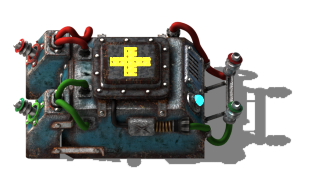
\includegraphics{pics/factorio-arithmetic.png}
\captionof{figure}{Combinateur arithmétique}
}


\end{minipage} 


\paragraph{}
Le combinateur arithmétique évalue des opérations arithmétiques à partir de ses signaux d'entrée et émet le résultat sur les signaux spécifiés dans l'emplacement de signal de sortie. 
L'entrée et la sortie peut se faire sur n'importe quel signal d'objet ou signal virtuel.

\paragraph{Branchements} 
Le combinateur arithmétique se connecte à un réseau rouge ou vert sur son coté \textbf{entrée} représenté par les terminaux font partie intégrante du combinateur et ressemblent a des branchements ampoules, et réalise une opération arithmétique qui sera émise à partir du coté \textbf{sortie} d'où les câbles de sortie semblent sortir un peu du combinateur. 

\paragraph{Retour de signal}
Notez que le réseau d'entrée et le réseau de sortie \textbf{ne sont pas le même réseau}.
Connecter le réseau de sortie au réseau d'entrée résultera en une boucle de retour. 

Par exemple, ajouter 1 à la valeur des plaques de cuivre et l'émettre en tant que plaques de cuivre est une action qui résultera en une boucle infinie si la sortie est connectée à l'entrée. 
La valeur des plaques de cuivre va alors vite (mais pas instantanément) augmenter. 
La vitesse à laquelle celle ci augmente est de 1 par mise à jour du moteur de jeu, autrement appelé \textbf{tick de jeu}. 

Cette technique peut être combinée avec la logique de combinateur logique pour réaliser des horloges électroniques, des portes, et d'autres systèmes;

\paragraph{Signal ['Chacun']}
Ce combinateur peut utiliser le signal ['Chacun'] à la fois en entrée et en sortie, auquel cas tous les signaux différents de zéro vont se voir calculés séparément selon l'opération du combinateur et leur résultat émis sur le coté sortie.
Avoir le signal ['Chacun'] à la fois en entrée et en sortie et utiliser une opération non modifiante (comme ajouter 0) est équivalent à un câble à sens unique; toutes les informations du réseau d'entrée est copiée au réseau de sortie, mais l'inverse n'est pas vrai.

\paragraph{Jonction de réseaux}
Les combinateurs arithmétiques peuvent être utilisés pour joindre deux réseaux sur leur coté entrée et renvoyer la somme de leurs réseaux.

\subsection{Le combinateur logique}
\begin{minipage}[t]{\textwidth}

{
\centering
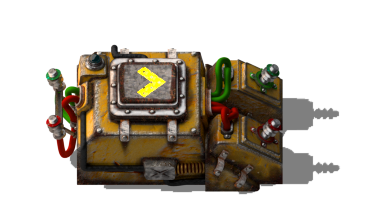
\includegraphics{pics/factorio-decider.png}
\captionof{figure}{Combinateur logique}
}

\end{minipage} 

\paragraph{}
Le combinateur logique fonctionne comme un combinateur arithmetique, mais est designé pour comparer des valeurs.
Essentiellement, c'est un conditionnel.

En termes de connexion, retour, et de signaux, il fonctionne tel que décris plus haut. De plus, il peut gérer les signaux ['Tout'] et ['N'importe quoi'], et permet de réaliser des comparaisons logiques. 

\subsection{L'émetteur de constante}
\begin{minipage}[t]{\textwidth}


{
\centering
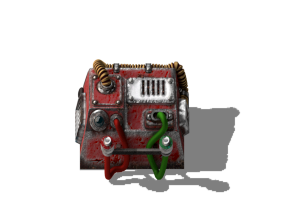
\includegraphics{pics/factorio-constant.png}
\captionof{figure}{Émetteur de constante}
}

\end{minipage}

\paragraph{}
L'émetteur de constante émet jusqu'à 15 valeurs sur n'importe quel signal sur tous les réseaux logiques qui y sont branchés. 
(Vous ne pouvez pas spécifier si une valeur devrait être envoyé sur le réseau rouge ou vert uniquement; si vous avez besoin de deux valeurs différentes, utilisez deux émetteurs, un pour chaque couleur de cable.) 
Vous pouvez utiliser n'importe quel signal d'objet ou n'importe quel signal virtuel.

\begin{info}
Notez qu'utiliser deux emplacements de signaux pour émettre des valeurs sur le même signal reviens à émettre la somme des deux valeurs sur un seul emplacement.
\end{info}